\begin{ESKDtitlePage}
  \begin{flushright}
    \textbf{ПРИЛОЖЕНИЕ Г} \enspace\enspace
  \end{flushright}
  
  \begin{center}
    % \envDiplomMinistr \\
    \envDiplomEducation \\
    \envDiplomUniversity \\
    \envDiplomCathedra \\
  \end{center}

  \vfill

  \begin{center}
    \textbf{ИНСТРУКЦИЯ ПО УСТАНОВКЕ ПО}
  \end{center}

  \vfill

  \begin{center}
    \envCode \\
  \end{center}

  \vfill

  \begin{flushright}
  \begin{minipage}[t]{.49\textwidth}
    \begin{minipage}[t]{.75\textwidth}
      \begin{flushright}
        \envDiplomTeacherInfo\\
        \hspace{0pt}\\
        \envDiplomStudentInfo\\
        \hspace{0pt}\\
        Консультанты:\\
        \envDiplomEspdInfo\\
        \hspace{0pt}\\
        \envDiplomRecendentInfo\\
      \end{flushright}
    \end{minipage}
  \end{minipage}
  \begin{minipage}[t]{.49\textwidth}
    \begin{flushright}
      \begin{minipage}[t]{.75\textwidth}
        \envDiplomTeacherInitials~\envDiplomTeacherSurname\\ % Руководитель
        \hspace{0pt}\\
        \envDiplomStudentInitials~\envDiplomStudentSurname\\ % Выполнил
        \hspace{0pt}\\
        \hspace{0pt}\\ % Консультанты:
        \envDiplomEspdInitials~\envDiplomEspdSurname\\ % по ЕСПД
        \hspace{0pt}\\
        \envDiplomRecendentInitials~\envDiplomRecendentSurname\\ % рецензент
      \end{minipage}
    \end{flushright}
  \end{minipage}
\end{flushright}


  \vfill

  \begin{center}
    \ESKDtheYear
  \end{center}
\end{ESKDtitlePage}


\newpage
\tableofcontents
\hspace{0pt}\\

% \newpage
% \ESKDstyle{title}
% \thispagestyle{plain}
% \pagestyle{plain}
% \hspace{0pt}

\newpage
\section{УСТАНОВКА РЕДАКТОРА КОДА}

\begin{enumerate}
    \item[1.] Заходим на Github в профиль <<VSCodium>> в репозиторий <<vscodium>>.
    \item[2.] Открываем Releases. Результат на рис.~\ref{fig:vscodium_1}.
    \item[3.] Скачиваем установщик (Например, VSCodiumSetup-x64-*.exe).
    \item[4.] Запускаем файл.
    \item[5.] Соглашаемся с лицензией. Жмём <<Next>>. Результат на рис.~\ref{fig:vscodium_2}.
    \item[6.] Выбираем папку для установки. Жмём <<Next>>. Результат на рис.~\ref{fig:vscodium_3}.
    \item[7.] Жмём <<Next>>. Результат на рис.~\ref{fig:vscodium_4}.
    \item[8.] Добавляем ассоциацию файлов, добавив галочку. Жмём <<Next>>. Результат на рис.~\ref{fig:vscodium_5}.
    \item[9.] Жмём <<Install>>. Результат на рис.~\ref{fig:vscodium_6}.
\end{enumerate}

\begin{figure}[!phtb]
    \centering

    \begin{minipage}{0.49\textwidth}
        \centering

        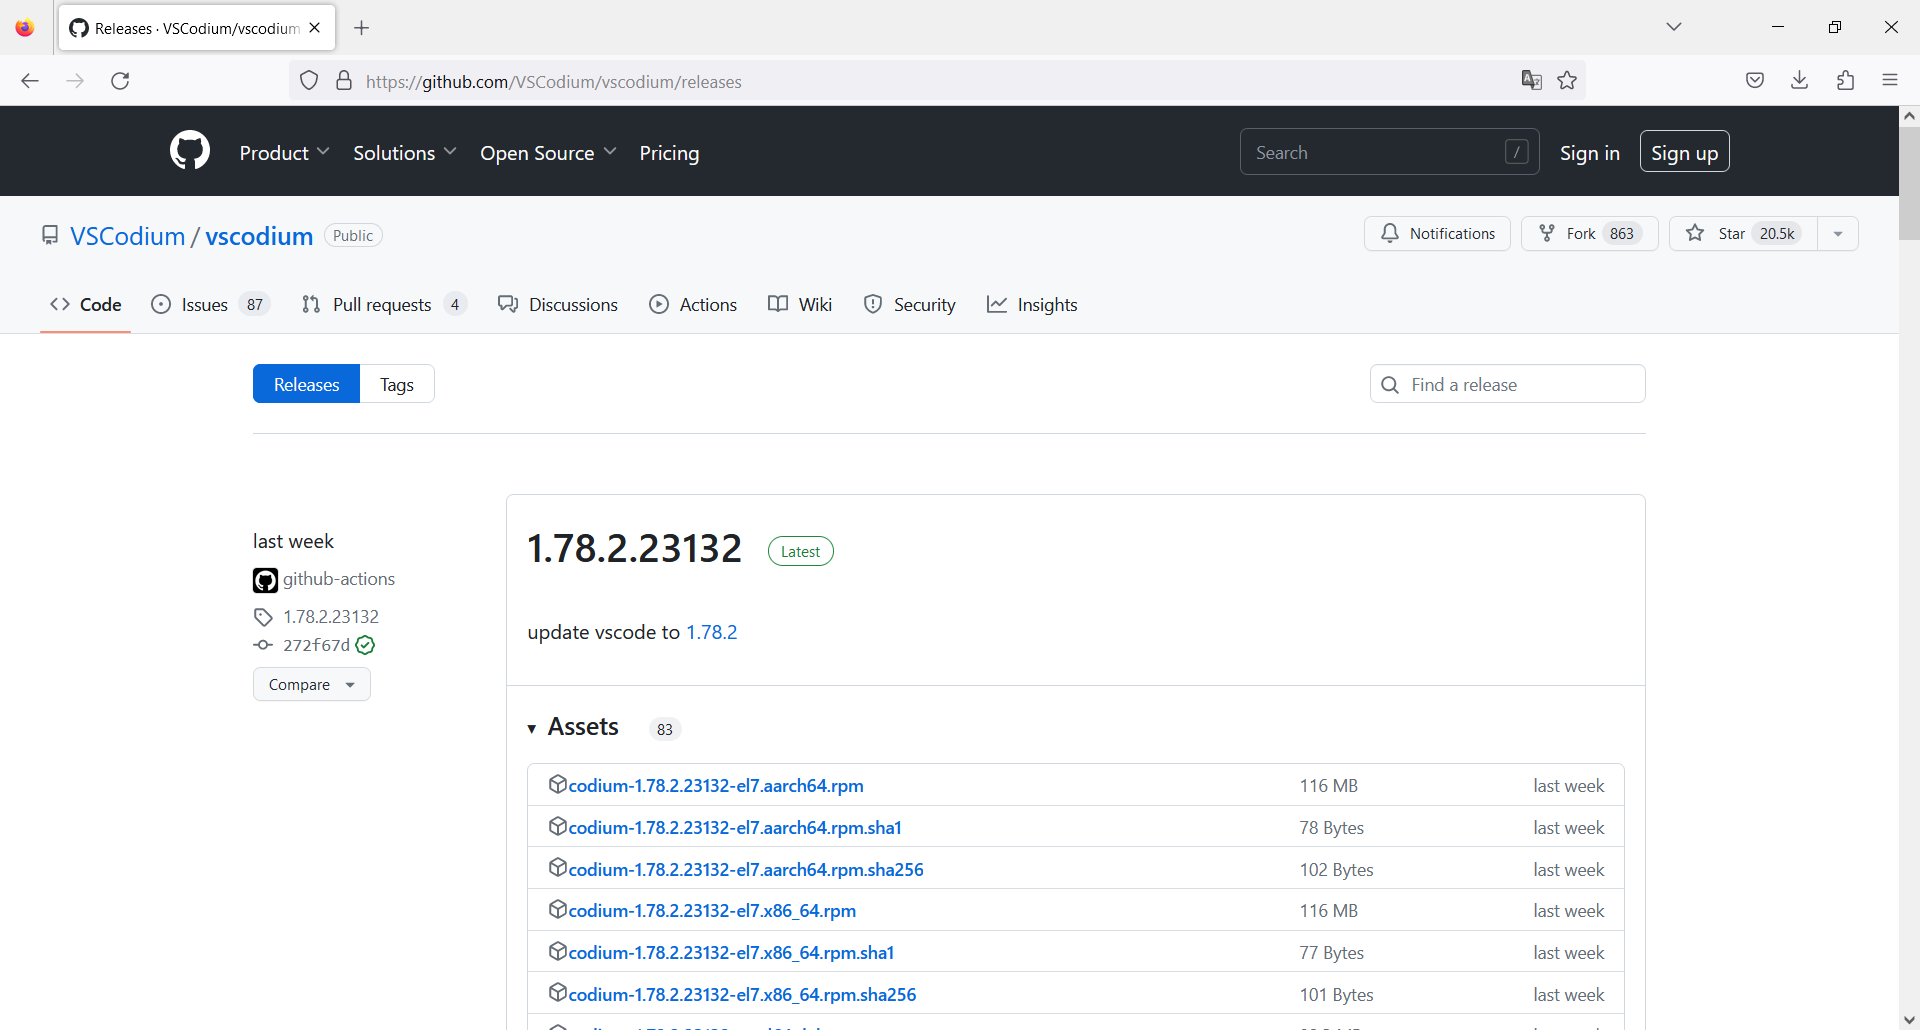
\includegraphics[height=5cm]
        {images/install/vs-codium/1.png}

        \caption{Скриншот}

        \label{fig:vscodium_1}
    \end{minipage}
    \begin{minipage}{0.49\textwidth}
        \centering

        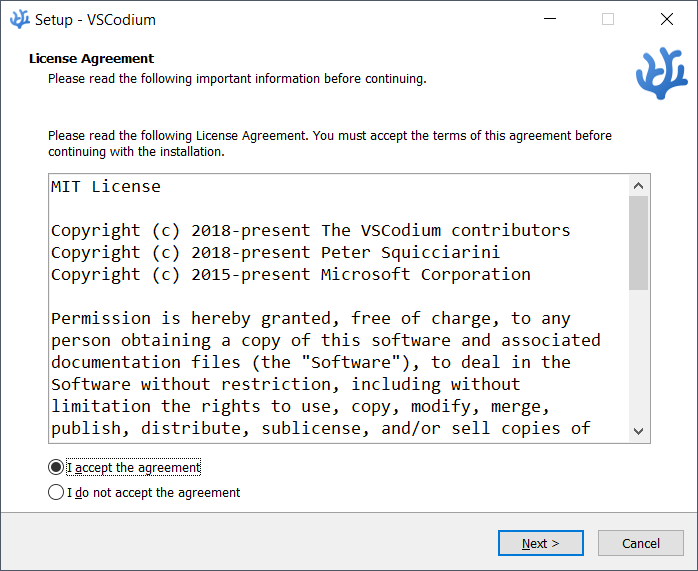
\includegraphics[height=5cm]
        {images/install/vs-codium/2.png}

        \caption{Скриншот}

        \label{fig:vscodium_2}
    \end{minipage}
\end{figure}

\begin{figure}[!phtb]
    \centering

    \begin{minipage}{0.49\textwidth}
        \centering

        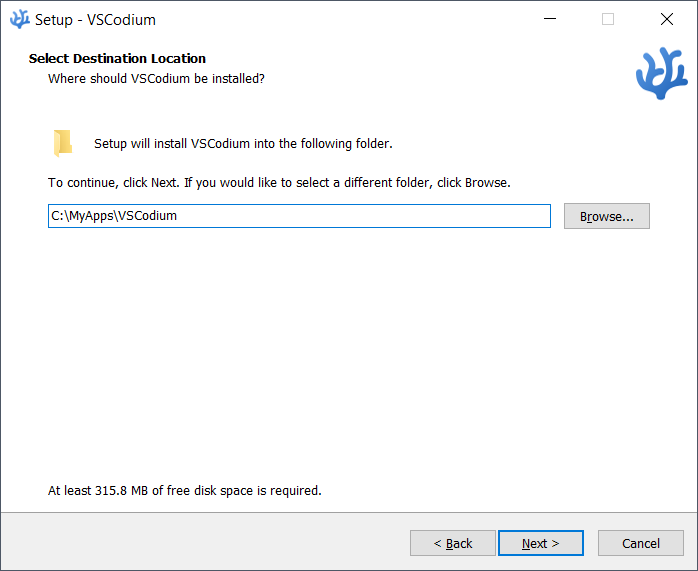
\includegraphics[height=5cm]
        {images/install/vs-codium/3.png}

        \caption{Скриншот}

        \label{fig:vscodium_3}
    \end{minipage}
    \begin{minipage}{0.49\textwidth}
        \centering

        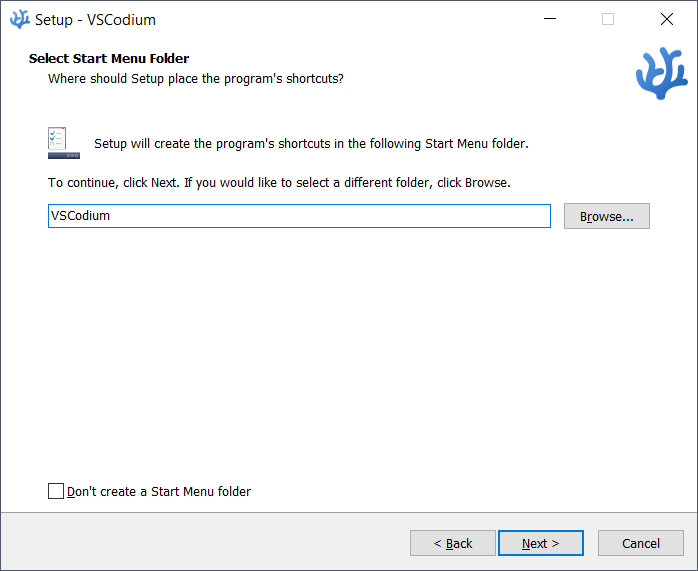
\includegraphics[height=5cm]
        {images/install/vs-codium/4.png}

        \caption{Скриншот}

        \label{fig:vscodium_4}
    \end{minipage}
\end{figure}

\begin{figure}[!phtb]
    \centering

    \begin{minipage}{0.49\textwidth}
        \centering

        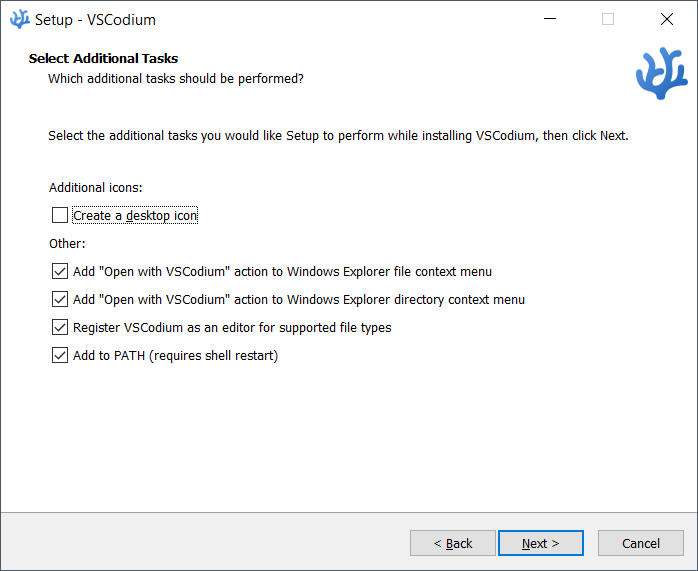
\includegraphics[height=5cm]
        {images/install/vs-codium/5.png}

        \caption{Скриншот}

        \label{fig:vscodium_5}
    \end{minipage}
    \begin{minipage}{0.49\textwidth}
        \centering

        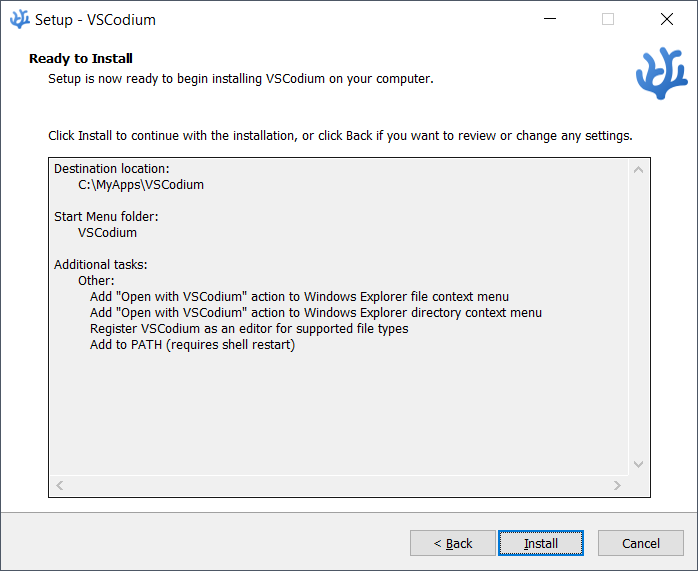
\includegraphics[height=5cm]
        {images/install/vs-codium/6.png}

        \caption{Скриншот}

        \label{fig:vscodium_6}
    \end{minipage}
\end{figure}

\section{УСТАНОВКА NODE JS}

\subsection{Установка NodeJS c пакетным менеджером npm}

\begin{enumerate}
    \item[1.] Заходим на сайт Node JS и выбираем для скачивания LST версию \ref{fig:nodejs_1}.
    \item[2.] Жмём <<Next>>. Результат на рис.~\ref{fig:nodejs_2}.
    \item[3.] Соглашаемся с лицензией. Жмём <<Next>>. Результат на рис.~\ref{fig:nodejs_3}.
    \item[4.] Выбираем папку для установки. Жмём <<Next>>. Результат на рис.~\ref{fig:nodejs_4}.
    \item[5.] Жмём <<Next>>. Результат на рис.~\ref{fig:nodejs_5}.
    \item[6.] Жмём <<Next>>. Результат на рис.~\ref{fig:nodejs_6}.
    \item[7.] Жмём <<Install>>. Результат на рис.~\ref{fig:nodejs_7}.
    \item[8.] Жмём <<Finish>>. Результат на рис.~\ref{fig:nodejs_8}.
    \item[9.] Для проверки корректности установки открываем командную строку <<Win>> + <<R>>, <<cmd>>, <<Enter>>.
    \item[10.] Вводим команду <<node -v>>. Если нет ошибки (вывелась версия, например, <<v18.16.0>>),
    то NodeJS установлен.
    \item[11.] Вводим команду <<npm -v>>. Если нет ошибки (вывелась версия, например, <<9.5.1>>),
    то пакетный менеджер npm установлен.
\end{enumerate}

\subsection{Установка пакетного менеджера yarn}

\begin{enumerate}
    \item[1.] Открываем командную строку <<Win>> + <<R>>, <<cmd>>, <<Enter>>.
    \item[2.] Вводим команду <<npm i -g yarn>>.
    \item[3.] Вводим команду <<yarn -v>>. Если нет ошибки (вывелась версия, например, <<1.22.19>>),
    то пакетный менеджер yarn установлен.
\end{enumerate}

\begin{figure}[!phtb]
    \centering

    \begin{minipage}{0.49\textwidth}
        \centering

        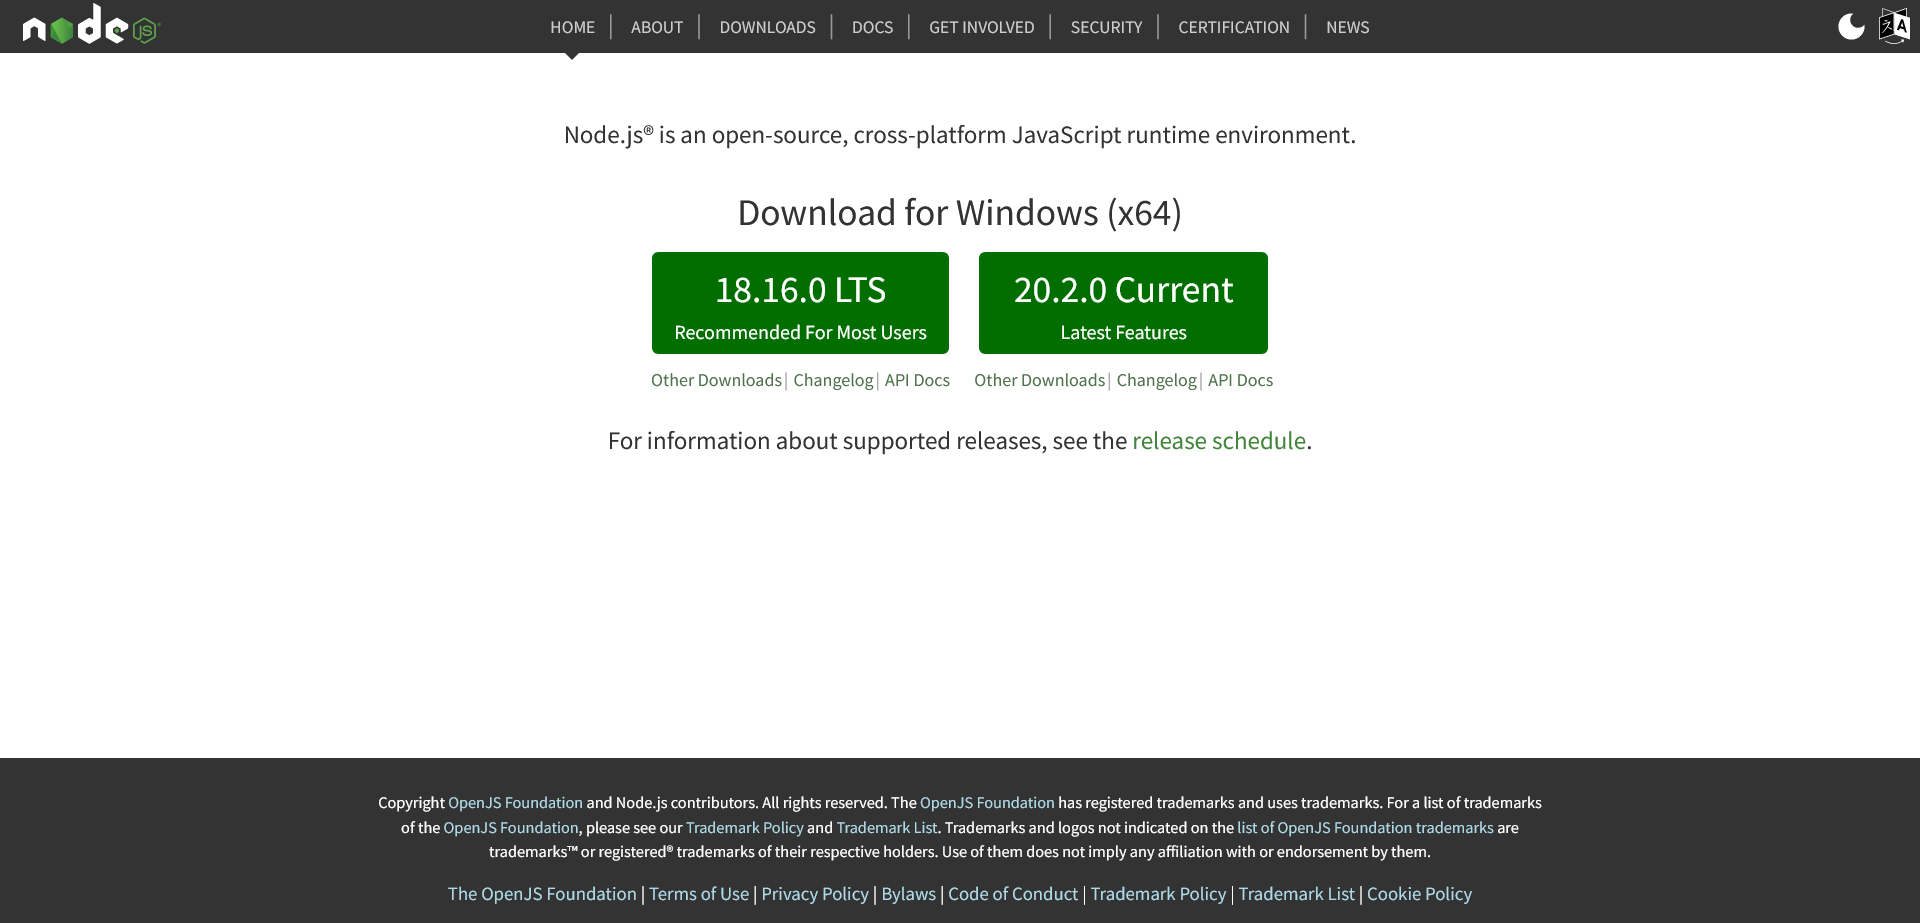
\includegraphics[height=4cm]
        {images/install/node-js/1.png}

        \caption{Скриншот}

        \label{fig:nodejs_1}
    \end{minipage}
    \begin{minipage}{0.49\textwidth}
        \centering

        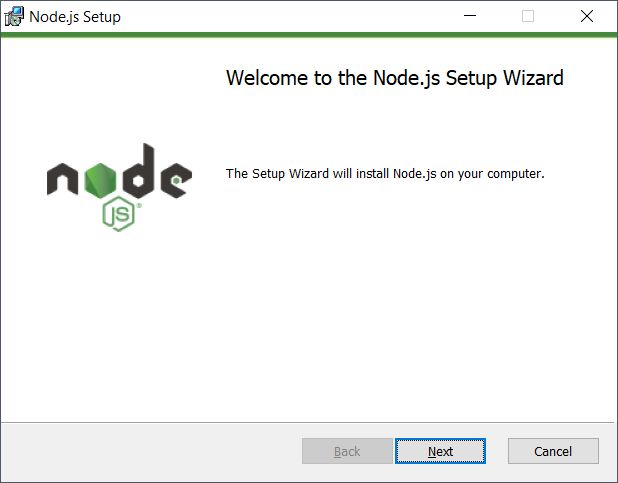
\includegraphics[height=4cm]
        {images/install/node-js/2.png}

        \caption{Скриншот}

        \label{fig:nodejs_2}
    \end{minipage}
\end{figure}

\begin{figure}[!phtb]
    \centering

    \begin{minipage}{0.49\textwidth}
        \centering

        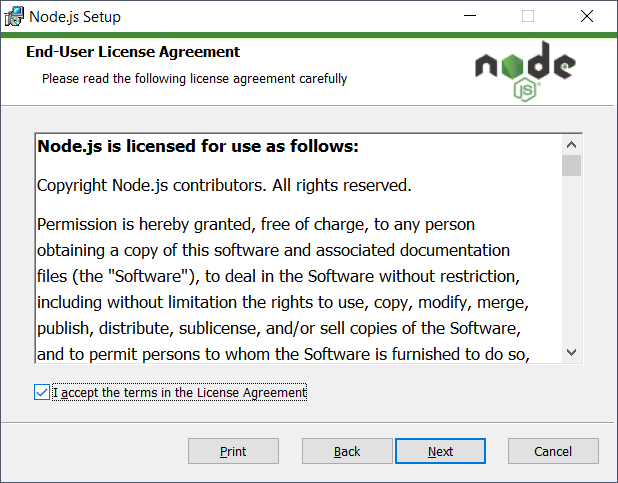
\includegraphics[height=5cm]
        {images/install/node-js/3.png}

        \caption{Скриншот}

        \label{fig:nodejs_3}
    \end{minipage}
    \begin{minipage}{0.49\textwidth}
        \centering

        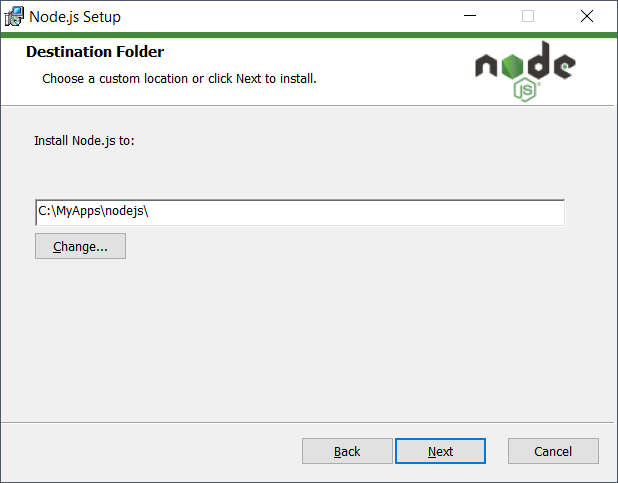
\includegraphics[height=5cm]
        {images/install/node-js/4.png}

        \caption{Скриншот}

        \label{fig:nodejs_4}
    \end{minipage}
\end{figure}

\begin{figure}[!phtb]
    \centering

    \begin{minipage}{0.49\textwidth}
        \centering

        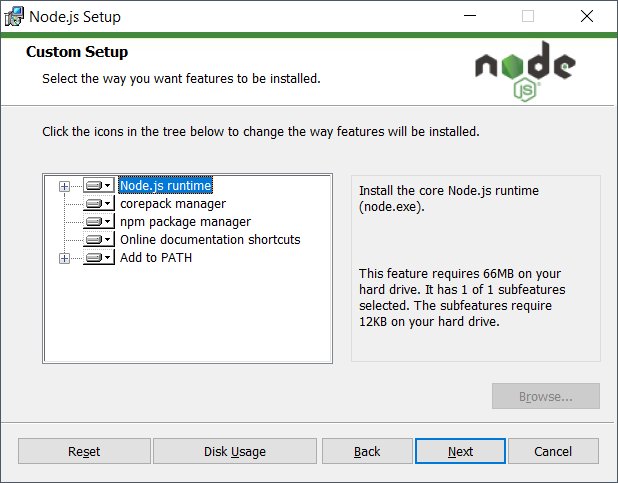
\includegraphics[height=5cm]
        {images/install/node-js/5.png}

        \caption{Скриншот}

        \label{fig:nodejs_5}
    \end{minipage}
    \begin{minipage}{0.49\textwidth}
        \centering

        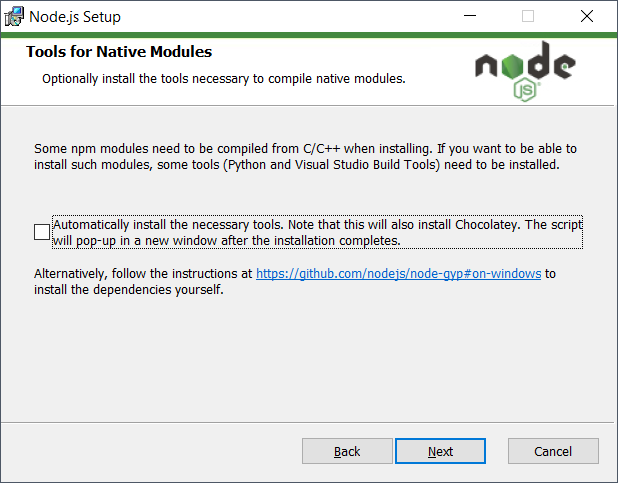
\includegraphics[height=5cm]
        {images/install/node-js/6.png}

        \caption{Скриншот}

        \label{fig:nodejs_6}
    \end{minipage}
\end{figure}

\begin{figure}[!phtb]
    \centering

    \begin{minipage}{0.49\textwidth}
        \centering

        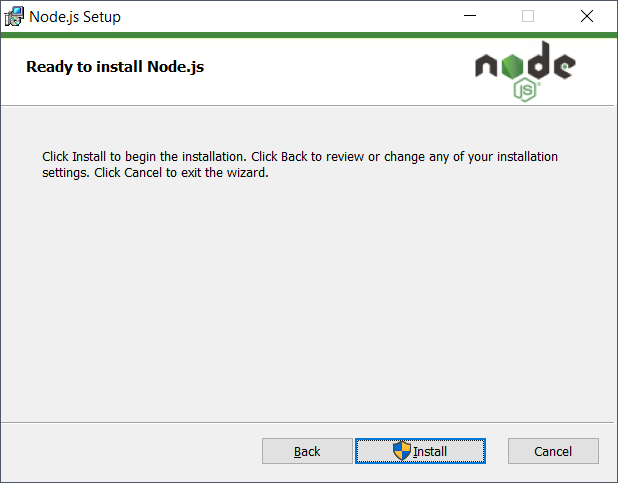
\includegraphics[height=5cm]
        {images/install/node-js/7.png}

        \caption{Скриншот}

        \label{fig:nodejs_7}
    \end{minipage}
    \begin{minipage}{0.49\textwidth}
        \centering

        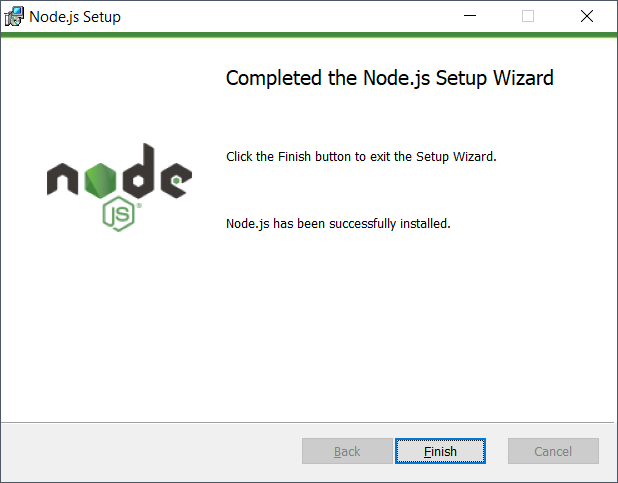
\includegraphics[height=5cm]
        {images/install/node-js/8.png}

        \caption{Скриншот}

        \label{fig:nodejs_8}
    \end{minipage}
\end{figure}

\newpage
\section{УСТАНОВКА DOCKER И DOCKER-COMPOSE}

\begin{enumerate}
    \item[1.] Заходим на сайт Docker и скачиваем установщик. Результат на рис.~\ref{fig:docker_1}.
    \item[2.] Запускаем установщик. Убираем галочку создания ярлыка на рабочем столе по желанию
    (ибо при каждом запуске компьютера нужно будет запускать Docker снова).
    Жмём <<OK>>.
    Результат на рис.~\ref{fig:docker_2}.
    \item[3.] Ждём установки. Результат на рис.~\ref{fig:docker_3}.
    \item[4.] Жмём <<Close and restart>>. Результат на рис.~\ref{fig:docker_4}.
    \item[5.] После перезапуска компьютера запускаем Docker.
    Жмём <<Accept>>.
    Результат на рис.~\ref{fig:docker_5}.
    \item[6.] Появилась предупреждение, что Docker работает с WSLv2, а у нас WSLv1.
    Результат на рис.~\ref{fig:docker_6}. Переходим по этой ссылке.
    \item[7.] Открылся сайт. Результат на рис.~\ref{fig:docker_7}.
    Нажимает на ссылку для скачивания установщика.
    \item[8.] Запускаем установщик. Жмём <<Next>>. Результат на рис.~\ref{fig:docker_8}.
    \item[9.] Жмём <<Finish>>. Результат на рис.~\ref{fig:docker_9}.
    \item[10.] Перезапускаем компьютер. Открываем Docker. Результат на рис.~\ref{fig:docker_10}.
    \item[11.] Для проверки корректности установки открываем командную строку <<Win>> + <<R>>, <<cmd>>, <<Enter>>.
    \item[12.] Вводим команду <<docker -v>>.
    Если нет ошибки (вывелась версия, например, <<Docker version 23.0.5>>), то Docker установлен.
    \item[13.] Вводим команду <<docker-compose -v>>.
    Если нет ошибки (вывелась версия, например, <<Docker-compose version 2.17.3>>), то docker-compose установлен.
\end{enumerate}

\begin{figure}[!phtb]
    \centering

    \begin{minipage}{0.49\textwidth}
        \centering

        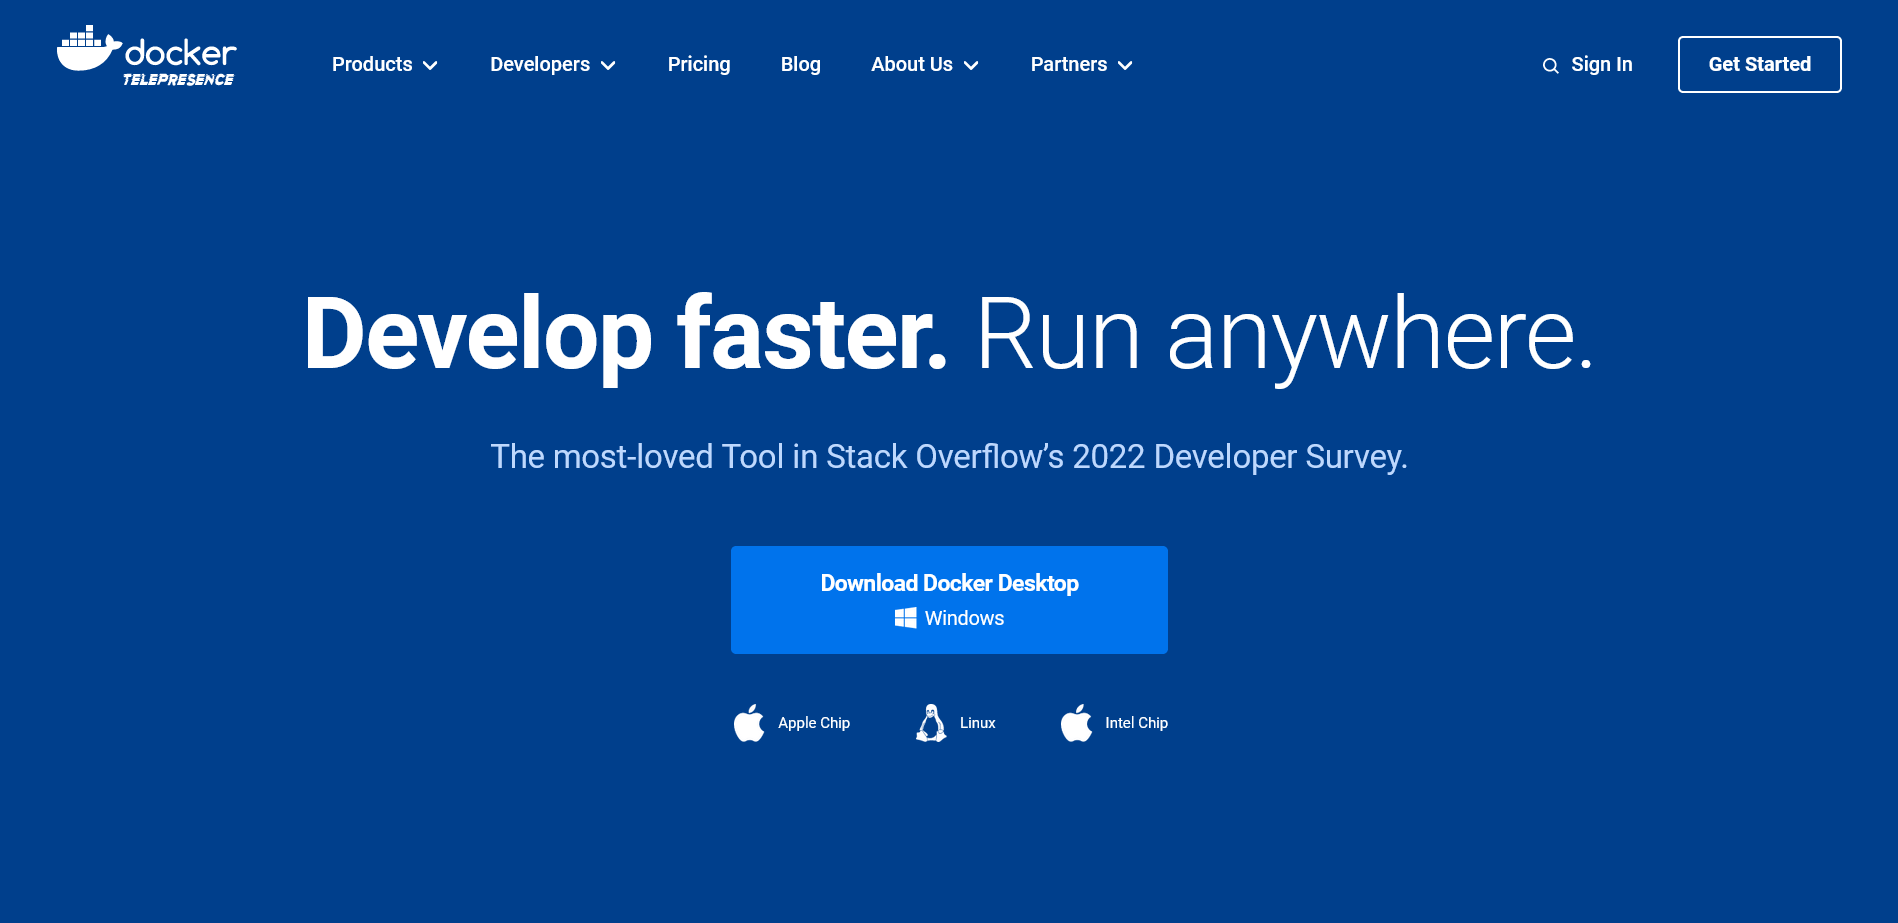
\includegraphics[width=0.99\textwidth]
        {images/install/docker/1.png}

        \caption{Скриншот}

        \label{fig:docker_1}
    \end{minipage}
    \begin{minipage}{0.49\textwidth}
        \centering

        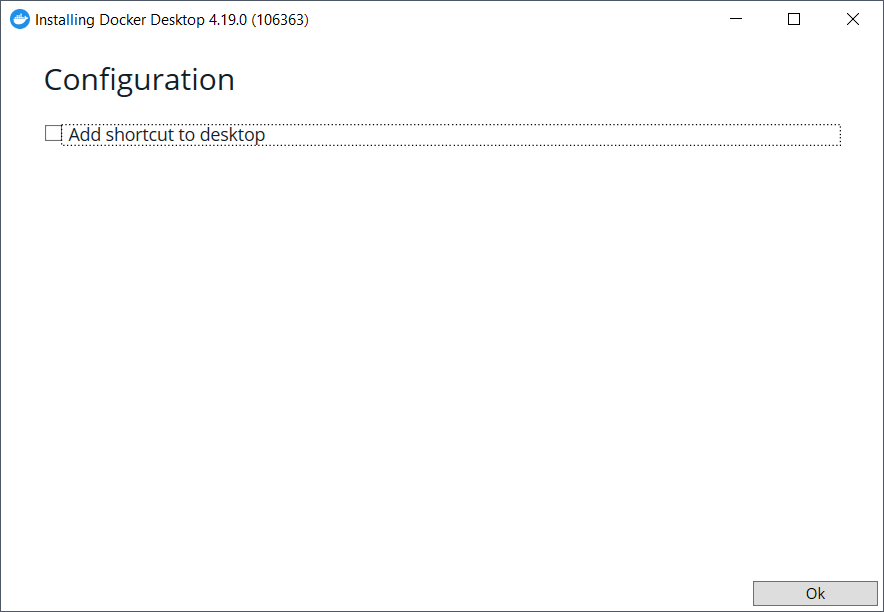
\includegraphics[height=5cm]
        {images/install/docker/2.png}

        \caption{Скриншот}

        \label{fig:docker_2}
    \end{minipage}
\end{figure}

\begin{figure}[!phtb]
    \centering

    \begin{minipage}{0.49\textwidth}
        \centering

        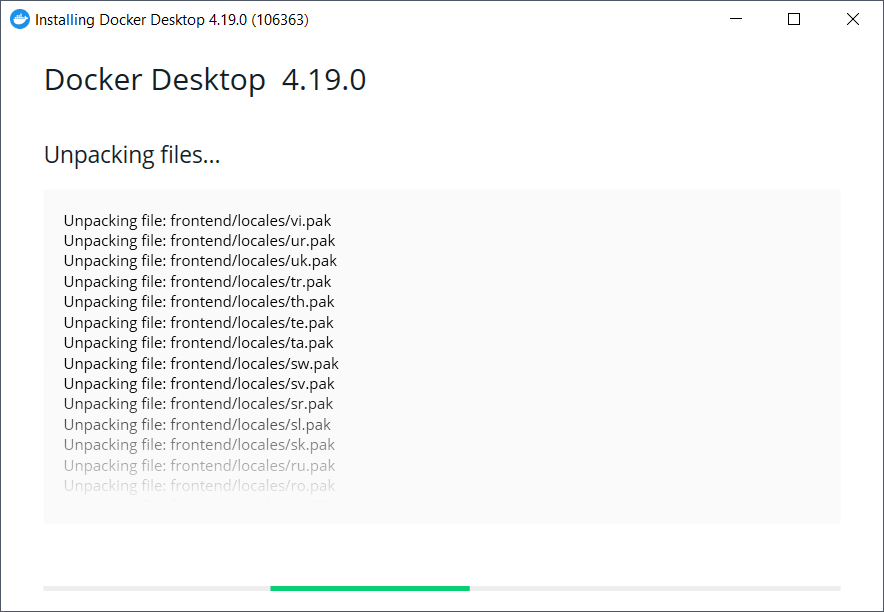
\includegraphics[height=5cm]
        {images/install/docker/3.png}

        \caption{Скриншот}

        \label{fig:docker_3}
    \end{minipage}
    \begin{minipage}{0.49\textwidth}
        \centering

        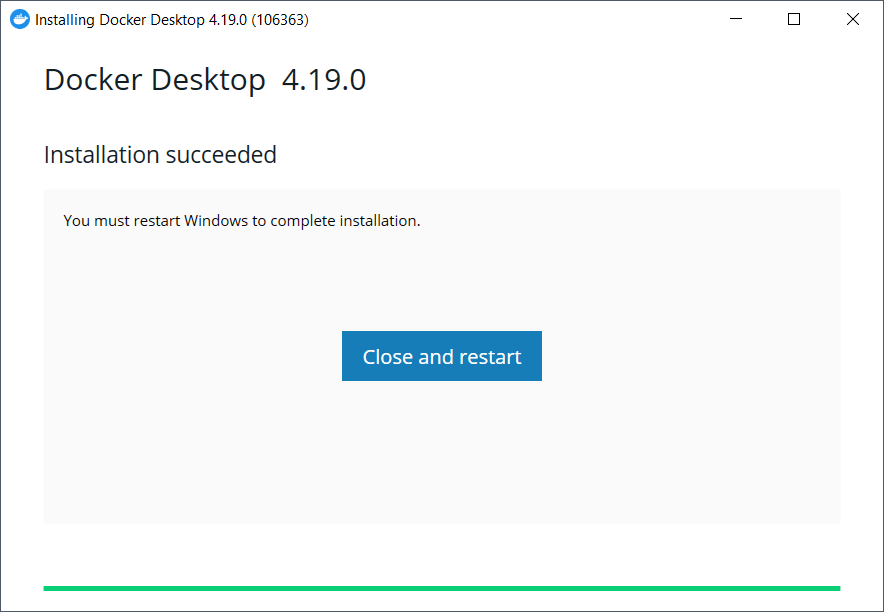
\includegraphics[height=5cm]
        {images/install/docker/4.png}

        \caption{Скриншот}

        \label{fig:docker_4}
    \end{minipage}
\end{figure}

\begin{figure}[!phtb]
    \centering

    \begin{minipage}{0.49\textwidth}
        \centering

        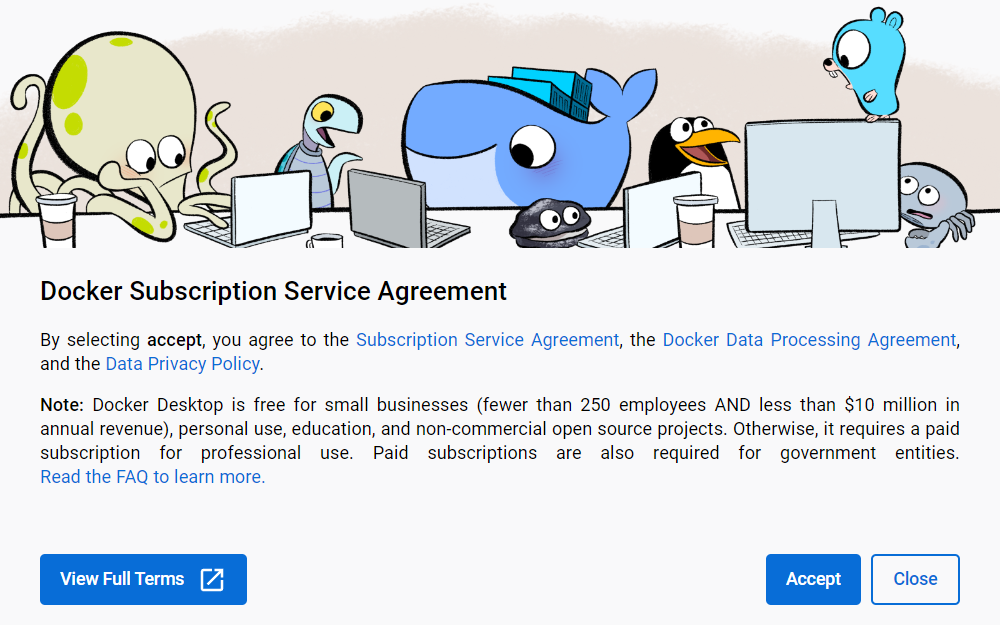
\includegraphics[height=5cm]
        {images/install/docker/5.png}

        \caption{Скриншот}

        \label{fig:docker_5}
    \end{minipage}
    \begin{minipage}{0.49\textwidth}
        \centering

        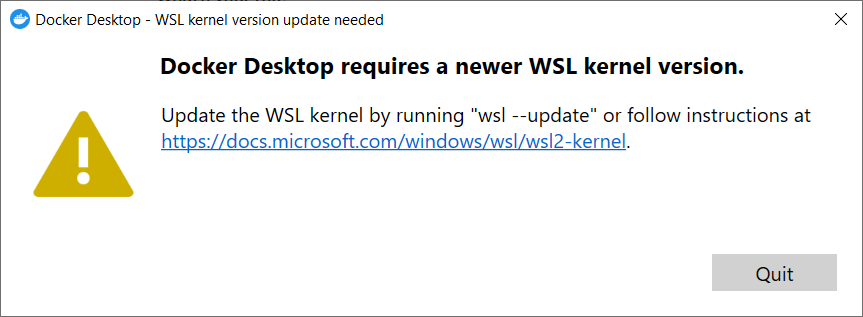
\includegraphics[width=0.99\textwidth]
        {images/install/docker/6.png}

        \caption{Скриншот}

        \label{fig:docker_6}
    \end{minipage}
\end{figure}

\begin{figure}[!phtb]
    \centering

    \begin{minipage}{0.49\textwidth}
        \centering

        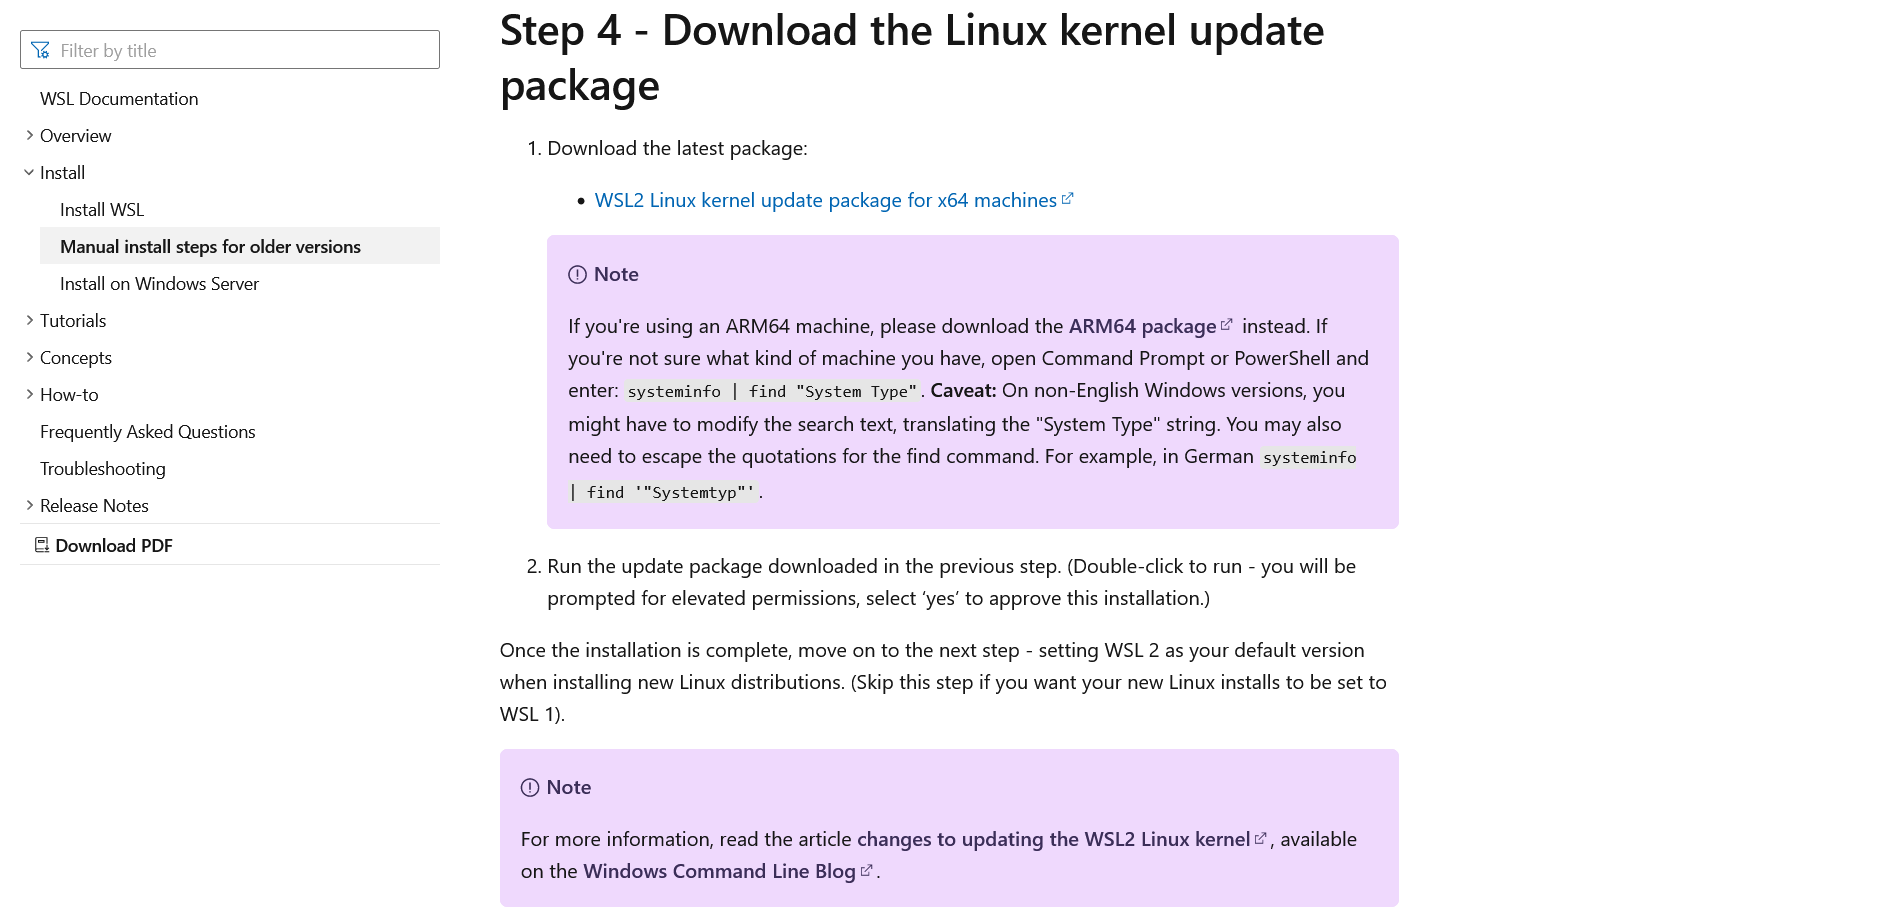
\includegraphics[height=5cm]
        {images/install/docker/7.png}

        \caption{Скриншот}

        \label{fig:docker_7}
    \end{minipage}
    \begin{minipage}{0.49\textwidth}
        \centering

        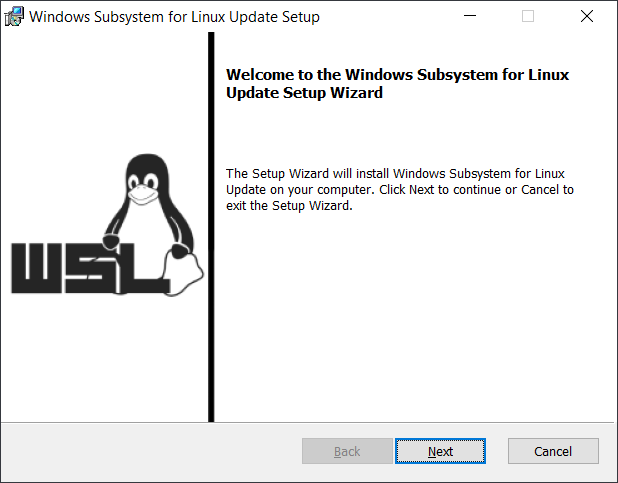
\includegraphics[height=5cm]
        {images/install/docker/8.png}

        \caption{Скриншот}

        \label{fig:docker_8}
    \end{minipage}
\end{figure}

\begin{figure}[!phtb]
    \centering

    \begin{minipage}{0.49\textwidth}
        \centering

        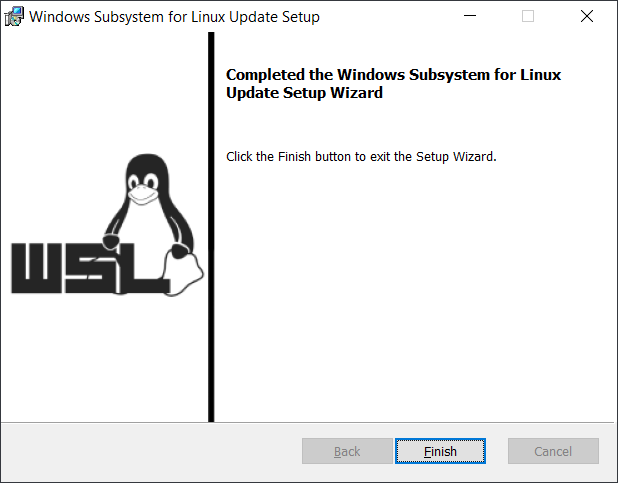
\includegraphics[height=5cm]
        {images/install/docker/9.png}

        \caption{Скриншот}

        \label{fig:docker_9}
    \end{minipage}
    \begin{minipage}{0.49\textwidth}
        \centering

        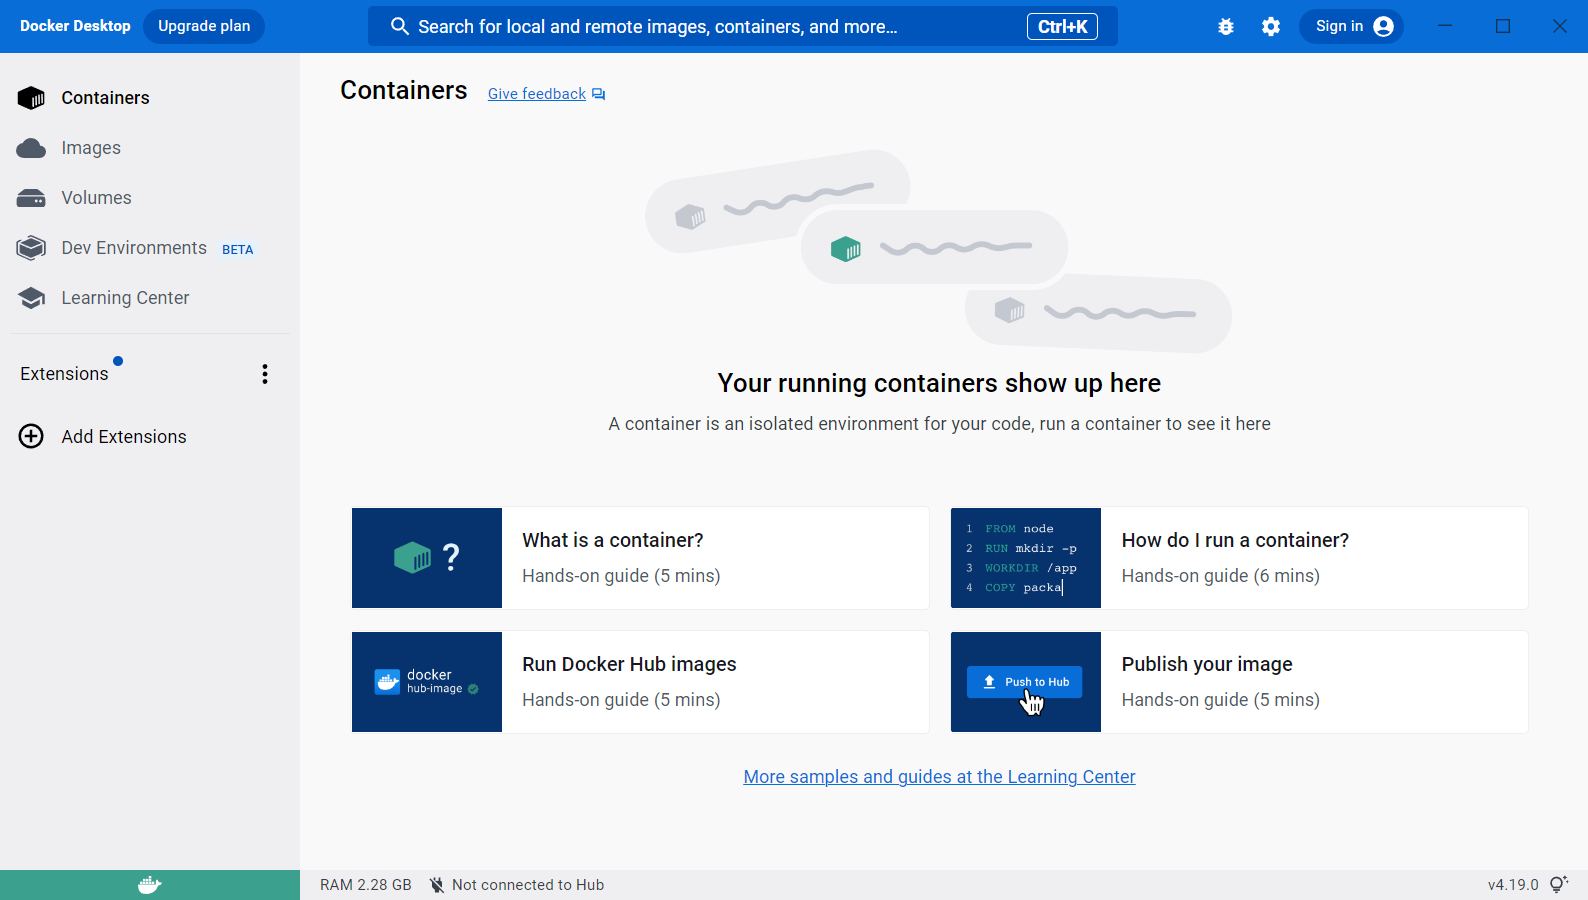
\includegraphics[height=5cm]
        {images/install/docker/10.png}

        \caption{Скриншот}

        \label{fig:docker_10}
    \end{minipage}
\end{figure}

\section{ЗАПУСК СЕРВЕРНОЙ ЧАСТИ ДЛЯ РАЗРАБОТКИ}

\subsection{Запуск MySQL и phpMyAdmin в Docker-контейнере}

Открываем папку <<dp\_backend>> (смотри папку на диске) в VS Codium.

\begin{enumerate}
    \item[1.] Жмём <<Terminal>>, <<New Terminal>>.
    \item[2.] Переходим папку с БД: <<cd docker>>, <<cd db>>, <<cd dev-mysql>>.
    \item[3.] Если нет файла <<.env>>, то создаем на основе <<.env.example>>.
    \item[4.] Запускаем контейнер командой <<docker-compose up>>.
\end{enumerate}

\subsection{Запуск миграций}

Папка <<dp\_backend>> открыта в VS Codium.

\begin{enumerate}
    \item[1.] Жмём <<Terminal>>, <<New Terminal>>.
    \item[2.] Переходим папку sources: <<cd sources>>.
    \item[3.] Если не установлены пакеты, устанавливаем командой <<yarn>>.
    \item[4.] Если не создан файл <<dev.env>>, то создаем на основе <<dev.env.example>>.
    \item[5.] Запускаем миграции командой <<yarn dev-migr-run>>.
\end{enumerate}

Откат миграции производится командой <<yarn dev-migr-rev>>.

Создание миграции производится командой <<yarn dev-migr-gen src/\\migrations/наименование>>.

\subsection{Запуск NestTS}

Папка <<dp\_backend>> открыта в VS Codium.

\begin{enumerate}
    \item[1.] Жмём <<Terminal>>, <<New Terminal>>.
    \item[2.] Переходим папку sources: <<cd sources>>.
    \item[3.] Если не установлены пакеты, устанавливаем командой <<yarn>>.
    \item[4.] Если не создан файл <<dev.env>>, то создаем на основе <<dev.env.example>>.
    \item[5.] Запускаем NestTS командой <<yarn dev-start>>.
\end{enumerate}
